% s

\documentclass[border=5pt, multi, tikz]{standalone}
\usepackage{tikz}

\begin{document}

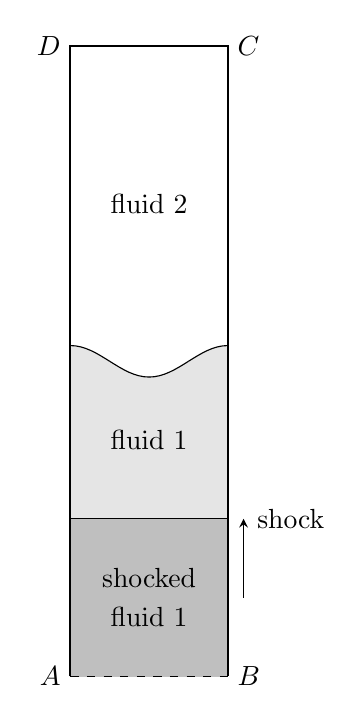
\begin{tikzpicture}
    %fill
    \filldraw[gray!20] (0,2) -- (0,4.2) cos (0.5,4) sin (1,3.8) cos (1.5,4) sin (2,4.2) -- (2,4.2) -- (2,2) -- cycle;
    \filldraw[gray!50] (0,0) -- (2,0) -- (2,2) -- (0,2) -- cycle;
    %grid cells
    \draw[thick] (0,0) -- (0,8) -- (2,8) -- (2,0);
    \draw[dashed] (0,0) -- (2,0);
    \draw (0,4.2) cos (0.5,4);
    \draw (0.5,4) sin (1,3.8);
    \draw (1,3.8) cos (1.5,4);
    \draw (1.5,4) sin (2,4.2);
    \draw (0,2) -- (2,2);
    \draw[->, >=stealth] (2.2,1) -- (2.2,2);
    %comments
    %\coordinate (f2) at (6,1);
    %\node at (f2) {fluid 2};
    \coordinate (A) at (0,0);
    \node at (A) [left] {$A$};
    \coordinate (B) at (2,0);
    \node at (B) [right] {$B$};
    \coordinate (C) at (2,8);
    \node at (C) [right] {$C$};
    \coordinate (D) at (0,8);
    \node at (D) [left] {$D$};
    \coordinate (shockedf1) at (1,1);
    \node at (shockedf1) [above] {shocked};
    \node at (shockedf1) [below] {fluid 1};
    \node at (1,3) {fluid 1};
    \node at (1,6) {fluid 2};
    \node at (2.8,2) {shock};
\end{tikzpicture}

\end{document}
